\chapter{Технологическая часть}

\section{Требования к программе}

К программе предъявляются следующие требования:

\begin{itemize}
	\item программа должна предоставлять пользователю возможность взаимодействовать со слаймом;
	\item оконный интерфейс программы должен предоставлять пользователю возможность изменять такие параметры слайма, как цвет, коэффициент пропускания и показатель поглощения;
	\item должна быть возможность перезагрузки сцены;
\end{itemize}

\section{Выбор инструментов разработки}

\section{Диаграмма классов}

\section{Интерфейс программы}

На рисунке \ref{ui} показан интерфейс программы.

\begin{figure}[H]
	\centering
	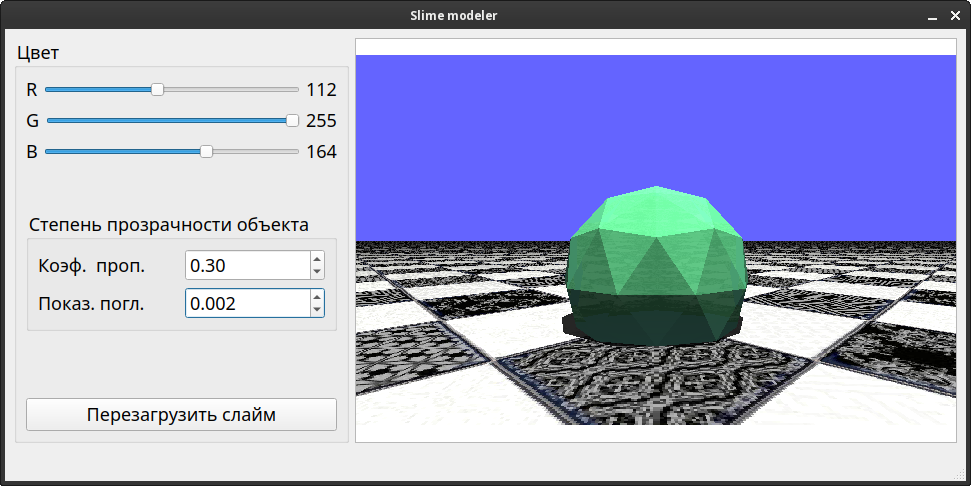
\includegraphics[width=\linewidth]{ui}
	\caption{Интерфейс программы}
	\label{ui}
\end{figure}

\clearpage
